\documentclass{llncs}
\usepackage{amsmath,amssymb,calc,ifthen}
\usepackage{float}
%\usepackage{cancel}
\usepackage[table,usenames,dvipsnames]{xcolor} % for coloured cells in tables
\usepackage{tikz}
% Allows us to click on links and references!
\usepackage{hyperref}
\usepackage{url}
\hypersetup{
colorlinks,
citecolor=black,
filecolor=black,
linkcolor=black,
urlcolor=black
}
% Nice package for plotting graphs
% See excellent guide:
% http://www.tug.org/TUGboat/tb31-1/tb97wright-pgfplots.pdf
\usetikzlibrary{plotmarks,shapes}
\usepackage{amsmath,graphicx}
\usepackage{epstopdf}
\usepackage{caption}
\usepackage{subcaption}
\usepackage{graphicx}
% highlight - useful for TODOs and similar
\usepackage{color}
\newcommand{\hilight}[1]{\colorbox{yellow}{#1}}
\newcommand\ci{\perp\!\!\!\perp} % perpendicular sign
\newcommand*\rfrac[2]{{}^{#1}\!/_{#2}} % diagonal fraction
\newcommand\SLASH{\char`\\}
\usepackage{listings}
% margin size
\usepackage{pdfpages}
\usepackage{enumitem} % for nested enumerate numbers 1 1.1 1.1.1
% \usepackage{breqn}
% \usepackage[linesnumbered]{algorithm2e}
% \usepackage{algorithmicx,algpseudocode}
% \usepackage{wrapfig} % for allowing text wrapped around the algorithm
% \newcommand\mycommfont[1]{\footnotesize\ttfamily\textcolor{blue}{#1}}
% \SetCommentSty{mycommfont}

% \usepackage{titlesec}
% \titlespacing*{\section}
% {0pt}{5.5ex plus 1ex minus .2ex}{4.3ex plus .2ex}


\DeclareMathOperator*{\argmin}{arg\,min}
\DeclareMathOperator*{\argmax}{arg\,max}

\begin{document}

\definecolor{blue3}{HTML}{86B7FC} % med blue
\definecolor{blue1}{HTML}{B5F1FF} % light blue
\definecolor{blue2}{HTML}{E0F9FF} % very light blue

\title{Disease Knowledge Transfer across Alzheimer's Variants}
%
\titlerunning{Disease Knowledge Transfer across Alzheimer's Variants}  % abbreviated title (for running head)
%                                     also used for the TOC unless
%                                     \toctitle is used
%

% * <mrazvan22@gmail.com> 2018-03-02T16:41:47.321Z:
% 
% Author list: Me, Marco (writing+model code), Pere (helped with validation), Alex (writing+tadpole), Neil (tadpole),  Arman, Keir (DTI data), Seb, Danny
% 
% ^ <mrazvan22@gmail.com> 2018-03-02T16:55:06.003Z.


\maketitle              % typeset the title of the contribution

\begin{abstract}

The availability of multimodal biomarker measurements in large scale clinical data is fundamental for the application of current disease progression models of neurodegenerative disorders. For this reason, disease progression modeling of rare dementias is currently very challenging, due to the presence of missing data and to the low sample size. To overcome this problem, in this study we introduce Disease Knowledge Transfer (DKT), a technique for transferring biomarker's progression models between Alzheimer's disease (AD) variants. We assume that different type of dementias affect overlapping brain regions ("Affected Overlap"), and thus present shared biomarker characteristics that can be transferred across diseases. We then implement this paradigm as a joint-disease generative model of biomarker progressions, disentangling disease-specific from  disease-agnostic biomarker relationships. We demonstrate DKT on independent datasets of 1) typical AD data (tAD), with large sample size and several biomarkers available over time, and 2) Posterior Cortical Atrophy (PCA) data, for which only MRI scans are available. DKT is able to predict, in testing PCA subjects, plausible population-level biomarkers for structural and molecular imaging biomarkers, for which no data was available. DKT may be a useful tool to analyse and understand rare forms of dementias for which multimodal data is not available or is limited. Moreover, by leveraging data from multiple diseases, DKT also has the potential to provide more accurate disease staging compared to traditional disease progression models.


\keywords{Disease Progression Model, Transfer Learning, Manifold Learning, Alzheimer's Disease, Posterior Cortical Atrophy}
\end{abstract}

\section{Introduction}


% biomarkers in alzheimer's -> measuring the evolution helps staging in clinical trials
Several image-based biomarkers for Alzheimer's disease (AD) are currently used to track the progression of the pathology: AV45 Positron Emission Tomography (PET) measuring amyloid-plaque aggregation, AV1451 PET measuring Tau tangle aggregation, Flourodeoxyglucose (FDG) PET measuring brain hypometabolism, Magnetic Resonance Imaging (MRI) measuring structural integrity and Diffusion Tensor Imaging (DTI) measuring connectivity integrity. Measuring the exact evolution of these biomarkers over the disease progression is fundamental for better understanding the pathology, as well as for improving the stratification in clinical trials through patient staging.

% hypothetical model -> dimention 1: ordering across modalities -> dimention 2: spatial ordering
A hypothetical model of disease progression has been previously published by \cite{jack2010hypothetical}, which proposes that the first biomarkers to become abnormal are measures of amyloid beta aggregation, followed by tau abnormalities, hypometabolism, structural MRI-based measures and finally cognitive decline. While this hypothetical model proposes a inter-modality ordering of biomarkers in typical AD, it has also been observed that within the same modality, biomarker measurements have a spatial sequence of abnormality that correlates with Braak stages: hippocampal volumes and entorhinal measures become abnormal first, followed by other structures within the temporal lobe, followed by parietal and frontal abnormalities.

Several data-driven methods have been proposed in order to reconstruct group-wise long term biomarker progressions from collections of short term individual biomarker measurements (\cite{lorenzi2017disease}, Young, Donohue). These approaches mostly rely on the estimation of a latent time reparameterization associated with each individual, often encoded by a translation (time shift) of the subject's measurements over the temporal axis.  This time reparameterization can be used as a proxy of disease staging associated with an individual biomarker profile relatively to the global disease progression model. 

% Flow: multimodal data needed for disease progression -> disease progression on rare dementias is challenging -> cannot apply model learned from other disease because of different spatial patterns -> but studies show at least some partial spatial overlap -> therefore transfer learning possible due to presence of "some overlap" -> benefits of transfer learning -> existing transfer learning literature
The availability of multimodal collections of biomarker's measurements across clinical groups is fundamental to the application of such disease progression models. For this reason, the application of disease progression modeling to rare dementia type is currently very challenging, due to the associated problem of missing biomarkers and low sample size.  Moreover, an average model of disease progression estimated from sporadic AD cases may not generalize to specific disease variants. For example, in Posterior Cortical Atrophy (PCA), posterior regions such as the occipital lobe and superior parietal regions have been shown to become affected early. While the spatial patterns are distinct between various forms of dementia, recent studies (Ossenkoppele, HBM, 2015) have showed at least partial spatial-overlap between different clinical phenotypes, while others have even suggested that PCA and typical AD subjects lie on a continuum of phenotypical variation \cite{crutch2012posterior}. The presence of overlap in pathology patterns across different dementias suggests that it should be theoretically possible to perform transfer learning across the diseases. There are two key benefits to performing transfer learning across dementia variants: 1. biomarker evolutions can be estimated for rare dementias for which there is not enough data (unimodal datasets, few subjects, cross-sectional data only) and 2. adding extra information from other datasets can help with staging and biomarker trajectory estimation. While recent studies \cite{hon2017towards} tried to transfer knowledge from generic image datasets to Alzheimer's disease, we are not aware of any studies that have tried to transfer knowledge across different types of Alzheimer's variants or other dementias. Furthermore, we are not aware of any studies to have done transfer learning in medical imaging for estimating a continuous disease progression without reliance on diagnostic classes, which are often biased.

% To overcome this problem, in this study we aim at defining a probabilistic framework for the estimation of disease progression trajectories in small datasets of specific disease subtypes, in presence of missing biomarkers and low numerosity. To this end we introduce the idea of \emph{transfer learning} of disease progression models across datasets. In particular, our framework is formulated in a probabilistic fashion, in order to quantify the uncertainty associated with low sample size and high variability characterizing the problem. 

We propose Disease Knowledge Transfer (DKT), a generative joint model that estimates continuous multimodal progressions for multiple dementias simultaneously and which inherently performs transfer learning between the modelled dementia phenotypes. This is achieved by disentangling \emph{disease-specific} from \emph{disease-agnostic} biomarker relationship. We fit the DKT model to three datasets simultaneously: (1) the TADPOLE Challenge dataset containing subjects from the ADNI study with MRI, FDG-PET, DTI, AV45 and AV1451 scans, (2) MRI scans from typical AD subjects in our local centre and (3) MRI scans from patients with Posterior Cortical Atrophy (PCA) from our local centre. We then used the fitted model to predict non-MRI trajectories for PCA patients, which have been learned from the multimodal TADPOLE dataset. We finally validated the DTI trajectories in PCA using a small test set of 20 DTI scans from the PCA patients and controls from our local centre.

% * <alexandra.young@ucl.ac.uk> 2018-03-02T17:54:07.562Z:
% 
% > unsupervised
% Is it unsupervised or does it know which disease/dataset is which, in which case it's semi-supervised?
% 
% ^ <mrazvan22@gmail.com> 2018-03-02T18:05:17.625Z:
% 
% Model is indeed supervised with respect to dataset/disease, but unsupervised with respect to diagnosis within same disease (e.g. Control, MCI and AD in ADNI). I removed the supervised-ness though in order not to create confusion. 
%
% ^.


\begin{figure}[h]
 \centering
 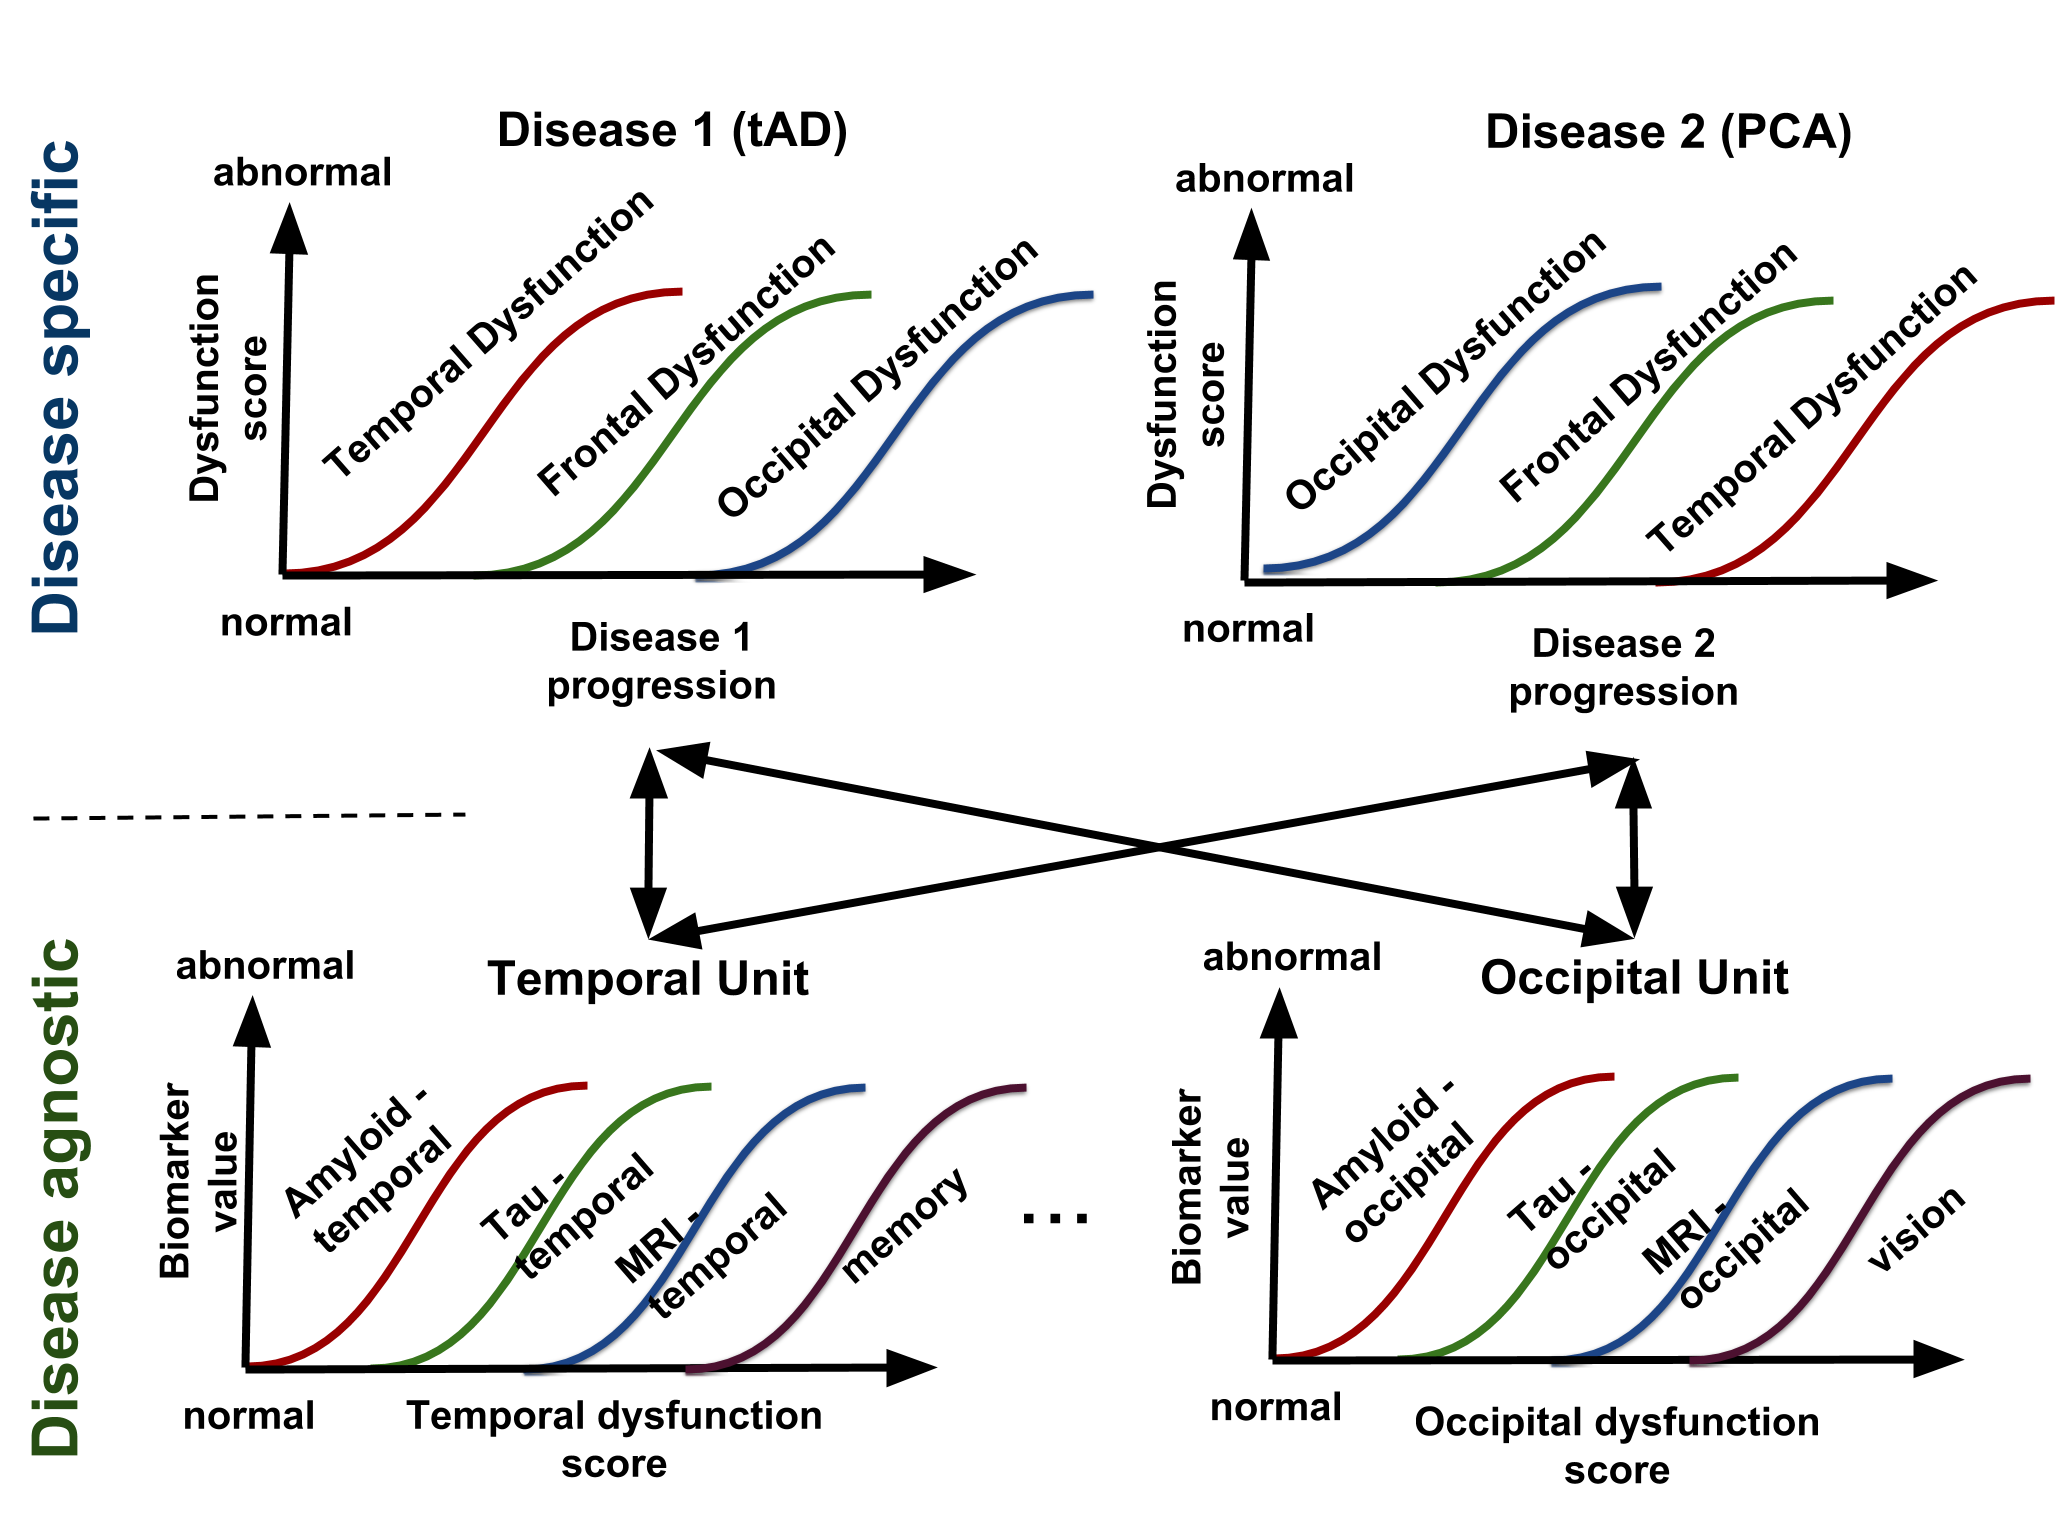
\includegraphics[width=\textwidth]{figures/disease_knowledge_transfer.png}
 \caption{Outline of the proposed framework for joint modelling of multiple diseases. We assume that each disease can be modelled as the evolution of abstract dysfunctionality scores, each related to different brain regions. Each dysfunctionality score is then assumed to be modelled as the progression of several biomarkers within that same region, but having different modalities. One key assumption of the model is that the biomarkers within each unit (bottom row) are disease agnostic (i.e. have the same dynamics for every disease), while the dysfunction scores (top row) are disease specific.}
 \label{fig:diagram}
\end{figure}

\subsection{Methods}

Fig. \ref{fig:diagram} shows the overall diagram of our proposed framework for joint modelling of disease. We assume that each disease can be modelled as the evolution of abstract dysfunctionality scores, each related to different brain regions (top row). Each dysfunctionality score is then assumed to be modelled as the progression of several biomarkers within that same region, but having different modalities (bottom row). Each group of biomarkers in the bottom row will be called a \emph{functional unit}, because the correlations between biomarkers are related though common "function" in a disease agnostic way, because they are related to the same underlying brain region. Biomarker groupings into functional units are defined a-priori. We model the correlations within each unit using a Gaussian-Process based disease progression model \cite{lorenzi2017disease}, for each region-specific functional unit we can model the correlation of biomarkers within that functional unit (Figure 1, bottom), which allows us to reconstruct a region- or unit-specific \emph{dysfunction} progression axis which can be used for staging subjects. Finally, we express the disease specific correlations (Figure 1, top) not directly with each biomarkers, but via the dysfunction scores estimated within each functional unit.  

The proposed model is parsimonious, easily interpretable by abstracting away biomarker information into the functional units, and can be used for \emph{disease knowledge transfer}, i.e. learning correlations in one disease from another. Our approach is inspired by transfer learning methods from machine learning, but the model is generative, easing interpretability.


Variable names:
\begin{itemize}
 \item $\Lambda$ = set of \emph{functional units}, i.e. \{temporal, parietal, occipital, ..\}. Biomarkers belonging to the same functional unit are asusmed to have disease-agnostic correlations.
 \item $y_{ijk}$ = measurement in subject $i$, visit $j$, biomarker $k$
%  \item $d_{ijl}$ = dysfunctionality score in subject $i$, visit $j$ in \emph{functional unit} $l$, where $l \in \Lambda$
%  \item $s_{ij}$ = disease progression score in subject $i$, visit $j$
 \item $\theta_k$ = parameters of trajectory for biomarker $k$
 \item $\lambda^l$ = parameters of trajectory for functional unit $l$, where $l \in \Lambda$
 \item $\psi$ : \{1, ..., K\} $ \rightarrow \Lambda$ is a function that maps beach biomarker to its corresponding functional unit
 \item $\beta_i$: time shift parameter for subject $i$ (disease specific)
 \item $\beta_i^{l}$: time shift parameter for subject $i$ used in functional unit $l$, where $l \in \Lambda$
 \item $\Omega$: set ${(i,j,k)}$ of measurements available from every subject $i$, visit $j$ in biomarker $k$
\end{itemize}

Likelihood for one single measurement in one subject visit: 
\begin{equation}
 p(y_{ijk}|\theta_k, \lambda^{\psi(k)}, \beta_i) = \sum_{\beta_i^{\psi(k)}} p(y_{ijk}| \beta_i^{\psi(k)}, \theta_k) p(\beta_i^{\psi(k)}| \lambda^{\psi(k)}, \beta_i)
\end{equation}

where $\beta_i^{\psi(k)}$ is a latent variable denoting the stage of subject $i$ in functional unit $\psi(k)$, where biomarker $k$ was assigned.

Extending the above to multiple, subjects, visits and biomarkers, we get the final model likelihood:
\begin{equation}
 p(y_{.,.,.}|\theta_1, ..., \theta_K, \{\lambda^{\psi(l)} | l \in \Lambda \}, \beta_1, ..., \beta_N) = \\ \prod_{(i,j,k) \in \Omega} \sum_{\beta_i^{\psi(k)}} p(y_{ijk}| \beta_i^{\psi(k)}, \theta_k) p(\beta_i^{\psi(k)}| \lambda^{\psi(k)}, \beta_i)
\end{equation}

Modelling of $p(y_{ijk}| \beta_i^{\psi(k)}, \theta_k)$ and $p(\beta_i^{\psi(k)}| \lambda^{\psi(k)}, \beta_i)$ will be done with a non-parametric model (Gaussian Process, Lorenzi et al., 2017)


Let's assume we have MRI and PET data in tAD (from ADNI), but only MRI data for another disease, e.g. PCA. We can model the disease-agnostic region-specific relationship between MRI and PET, and also build the disease specific progression models for tAD (using MRI and PET) and PCA (using MRI only). Finally, our model allows us to propagate the knowledge of PET dynamics in tAD to PCA subjects, without using any PET scans from PCA patients. This can be done by maximising the following likelihood (assuming we already have a model for tAD):

\begin{equation}
 p(y_{.,.,.}^{PCA}|\theta_1^{tAD}, ..., \theta_K^{tAD}, \{\lambda^{\psi(l)^{PCA}} | l \in \Lambda \}, \beta_1^{PCA}, ..., \beta_N^{PCA}) = 
\end{equation}

 \begin{equation}
 \prod_{(i,j,k) \in \Omega} \sum_{\beta_i^{\psi(k)}} p(y_{ijk}^{PCA}| \beta_i^{\psi(k)}, \theta_k^{tAD}) p(\beta_i^{\psi(k)}| \lambda^{\psi(k)^{PCA}}, \beta_i^{PCA})
\end{equation}

\section{Results}

% Fig1: biomarker traj. over dysfunction scores in one functional unit -> Fig2: dysfunction trajectories over disease stage in the two disease models -> Fig3: inferred biomarker trajectories "directly" over disease stage  in PCA
Fig. \ref{fig:occipUnit} shows the estimated biomarker trajectories within the \emph{occipital unit} plotted over the dysfunction scores, along with samples from the model posterior and aligned subject data. The X-axis shows the dysfunctionality scores within the occipital unit, which represent estimated time-shifts, in months, from an arbitrary reference X=0, while the Y-axis shows biomarker values normalised to [0,1] range. The model shows a good data fit, and we can observe most PCA subjects having abnormal occipital volumes, thus leading to high occipital dysfunctionality scores, in line with the current understanding of PCA as affecting posterior regions \cite{crutch2012posterior}. Fig. \ref{fig:occipUnit} shows the progression of dysfunctionality scores over the disease stage for (a) typical AD and (b) PCA. In typical AD, we see that temporal dysfunction becomes abnormal earliest, while PCA shows early parietal dysfunction, again in line with previous findings in the literature \cite{crutch2012posterior} (J.C. Baron, Neuroimage, 2001). In Fig. \ref{fig:PCAtrajByModality}, we plot the inferred biomarker trajectories for PCA directly across the disease progression. We do this for five different modalities: MRI Volumes, DTI, FDG, AV45 and AV1451. The results again recapitulate known patterns in PCA, where trajectories from posterior regions become abnormal first in MRI, DTI and AV1451, although in FDG we instead see temporal and hippocampal regions more affected. This might be due to the normalisation of the FDG trajectories on the Y-axis to the [0,1] range, which results in less scaling to trajectories that contain more disease signal. 

\newcommand{\expFld}{figures}

% data fitting within one unit
\begin{figure}
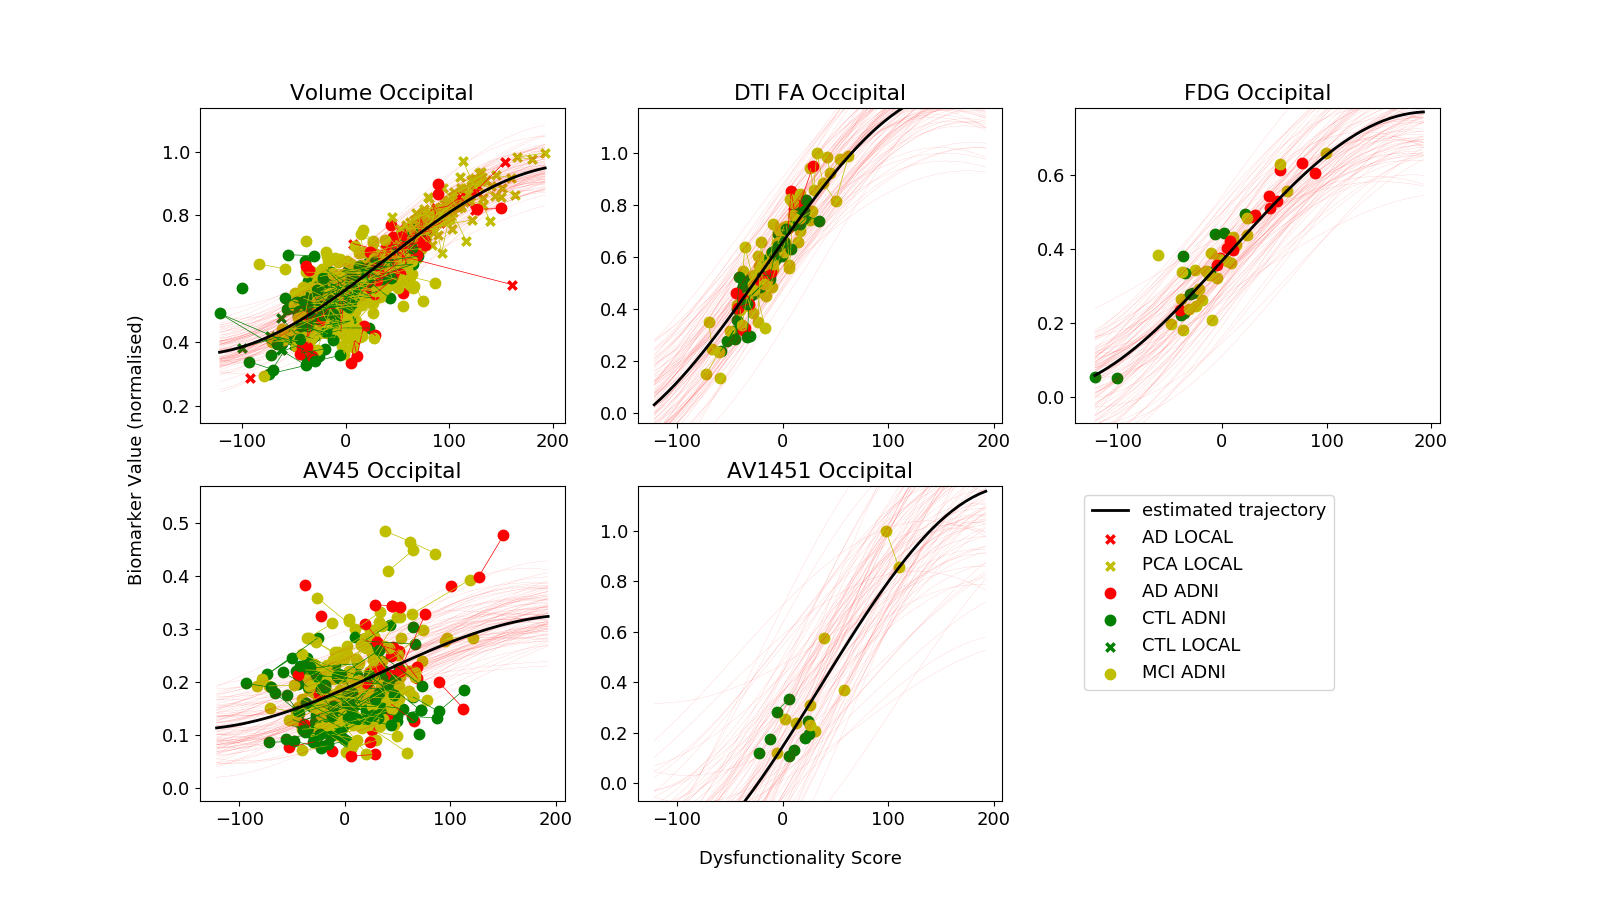
\includegraphics[width=\textwidth, trim=90 0 110 0, clip]{figures/unit1_allTraj_tad-drcTinyPen1_JMD.png} 
\caption{Estimated biomarker trajectories in the Occipital Unit. Subject data from ADNI and our local cohort are also shown. The X-axis represents, defined as the occipital dysfunctionality score, represents the time-shifts (in months) of each subject. Red lines represent samples from the trajectory posterior. The Y-axis measures biomarker values (normalised).}
\label{fig:occipUnit}
\end{figure}

% PCA vs tAD disease space
\begin{figure}
\begin{subfigure}{0.47\textwidth}
\centering
typical AD\\
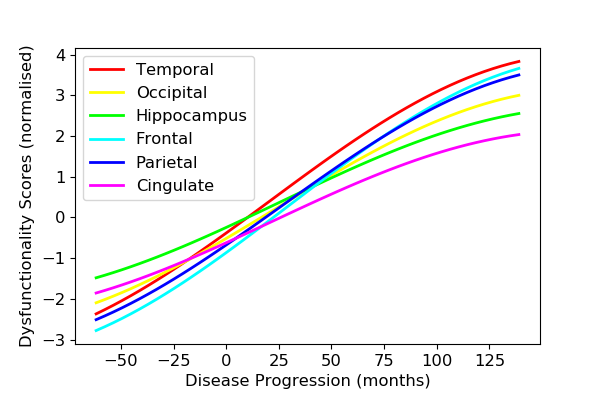
\includegraphics[width=\textwidth, trim=0 0 0 20, clip]{figures/tAD_trajSameSpace_tad-drcTinyPen1_JMD.png} 
\caption{}
\end{subfigure}
\begin{subfigure}{0.47\textwidth}
\centering
PCA\\
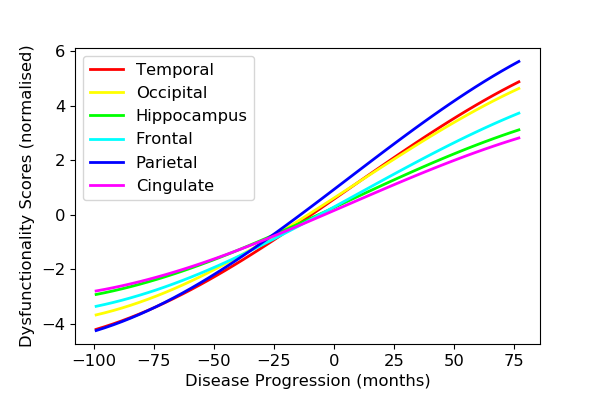
\includegraphics[width=\textwidth, trim=0 0 0 20, clip]{figures/PCA_trajSameSpace_tad-drcTinyPen1_JMD.png} 
\caption{}
\end{subfigure}
\caption{Progression of dysfunctionality scores for (a) typical AD and (b) PCA. In typical AD, we notice that the temporal scores are most affected after the disease }
\label{fig:pcaTadDisSpace}
\end{figure}



% estimated (hypothetical) trajectories in PCA: DTI, FDG, AV45, AV1451.Volumetric trajectories were based on PCA MRI data.
\begin{figure}[H]
 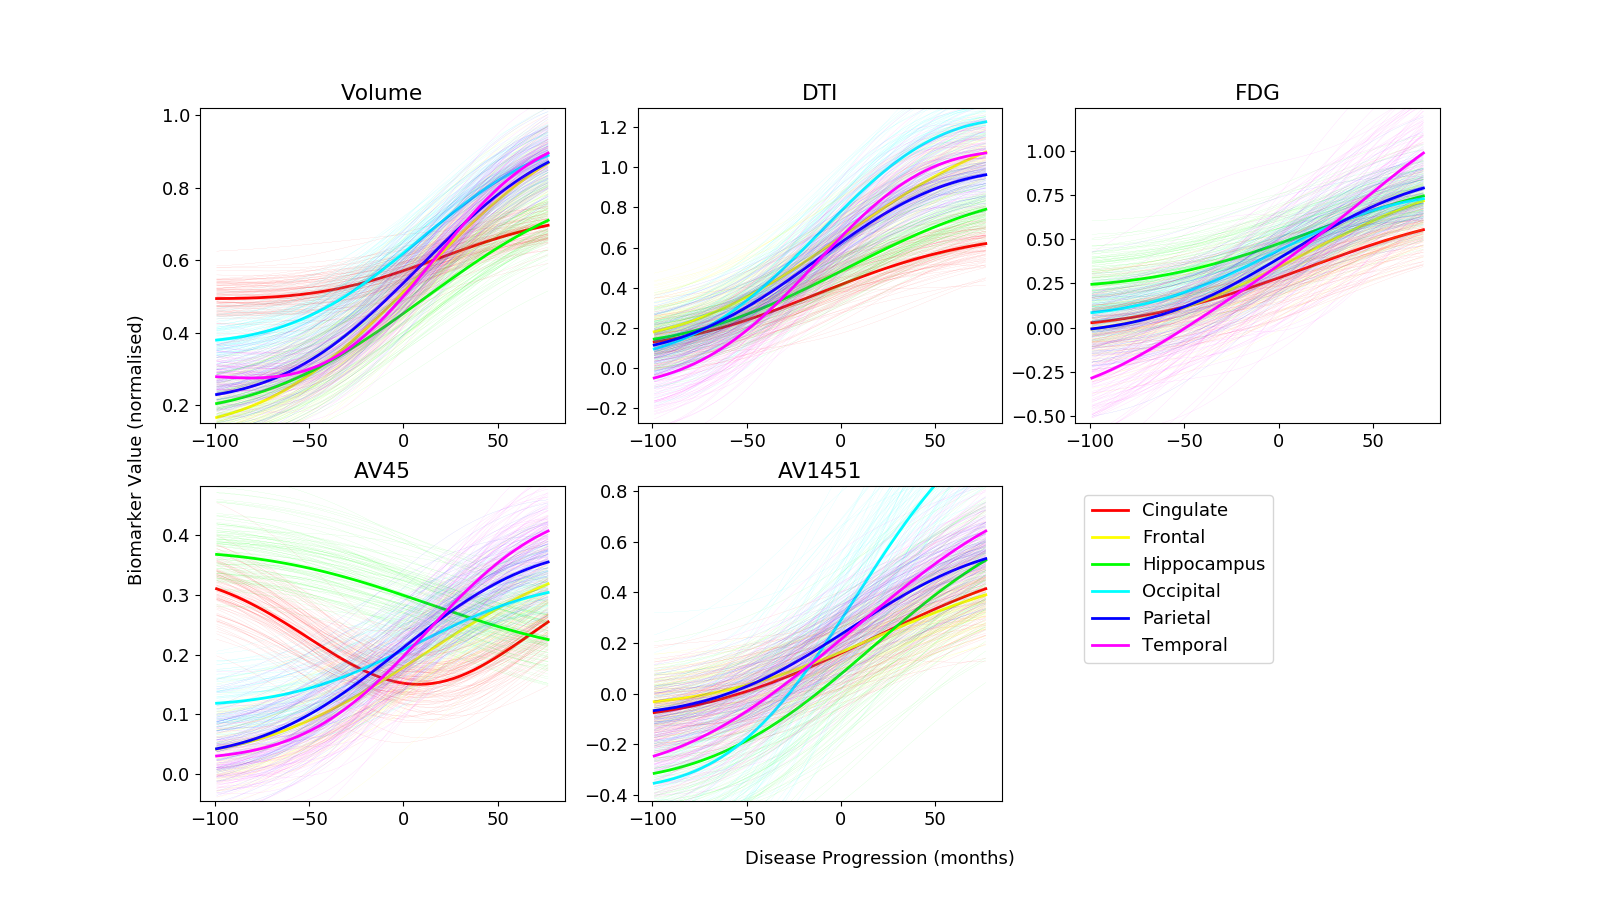
\includegraphics[width=\textwidth, trim=0 0 0 0, clip]{figures/trajDisSpaceOverlap_PCA_tad-drcTinyPen1_JMD.png}
 \caption{Estimated trajectories for the PCA cohort. The only data that was available was the MRI volumetric data. The dynamics of the other biomarkers has been inferred by the model using data from typical AD, and taking into account the different spatial distribution of pathology in PCA as compared to typical AD.}
 \label{fig:PCAtrajByModality}
\end{figure}
% * <mrazvan22@gmail.com> 2018-03-02T15:58:16.565Z:
% 
% two trajectories in AV45 screwed up due to bad initial starting point. Will take around 2-3h to fix, by implementing a more informed starting point, and re-fit the model. I'll try to see if I have time, otherwise might drop that modality?! Or take out the plot entirely.
% 
% ^.


\section*{Validation}

We performed validation using a separate test set of 20 DTI scans from controls and PCA patients from our local cohort. Fig. \ref{fig:DTIvalid} shows the estimated DTI biomarker trajectories plotted directly against the disease progression time-shifts, along with the DTI data from the test set. The time shift of each subject was estimated only based on their MRI scans. The inferred trajectories in PCA show good agreement with the data in the cingulate, hippocampus and temporal lobes, but less agreement in the other regions. This might be because the dataset that was used to train the model had better disease signal in DTI regions more traditionally associated with typical AD.

% LOCAL DTI validation

\begin{figure}[H]
 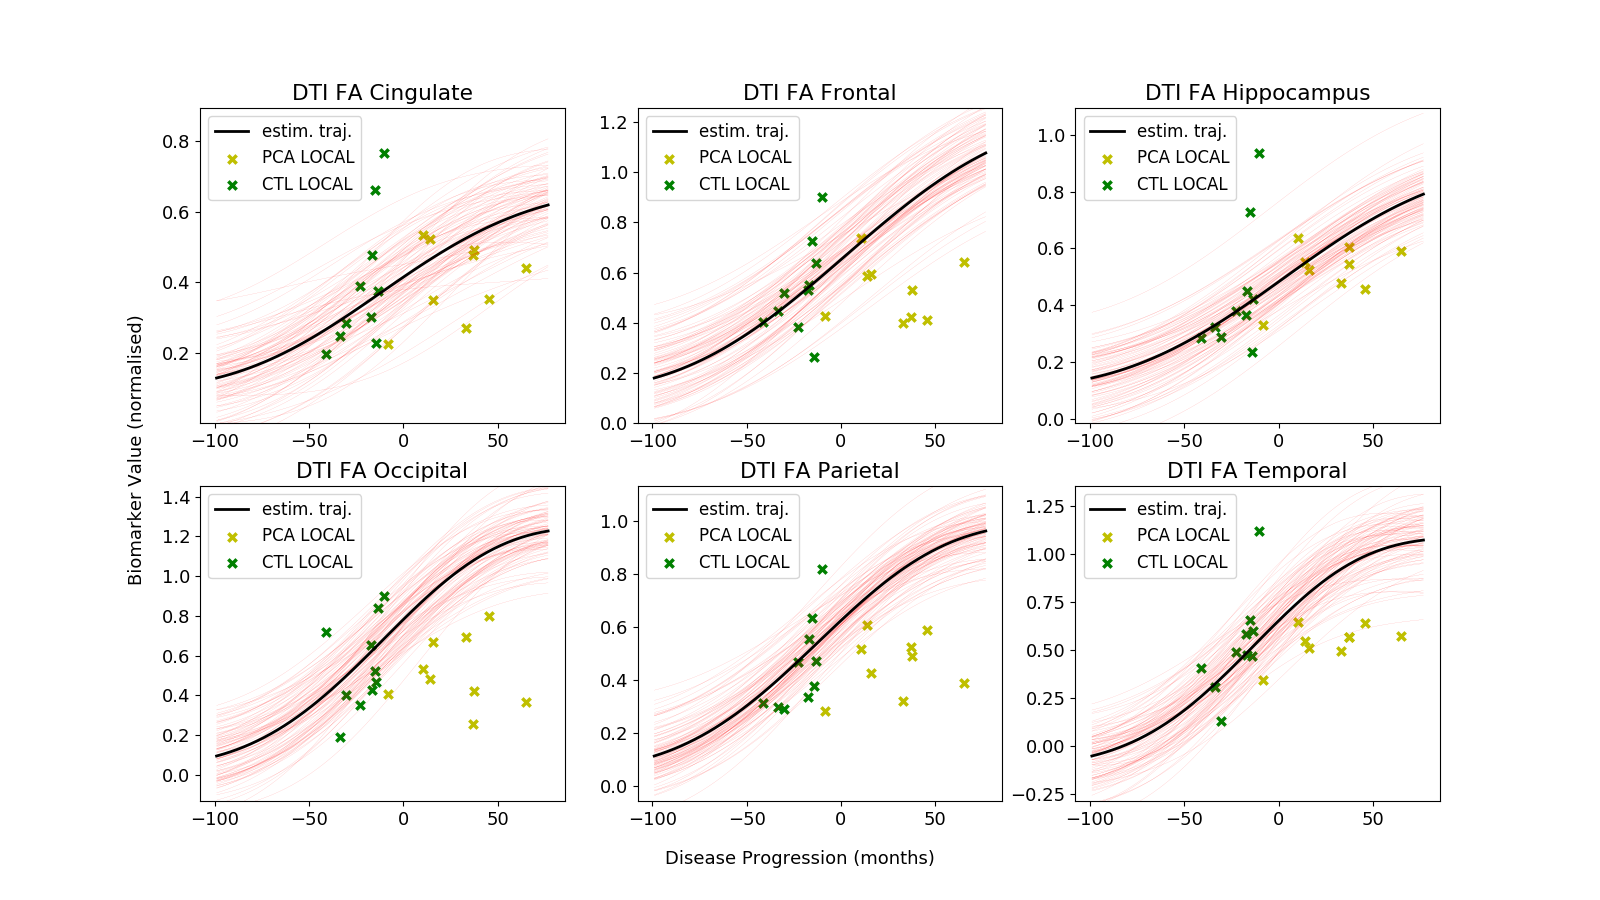
\includegraphics[width=\textwidth, trim=0 0 0 0, clip]{figures/validDtiPCA.png}
 \caption{Validation of the Disease Knowledge Transfer Model using DTI data of PCA subjects from our local cohort. Each subject has been shifted along the X-axis only according to their MRI data. No DTI data from PCA subjects was used to fit the model.}
\label{fig:DTIvalid}
\end{figure}

\section{Discussion}

% summary: what we developed -> what the model can do
We present here, for the first time, a framework for joint modelling of biomarker progression in multiple dementias simultaneously. The framework allows transferring biomarker trajectories to rare dementias for which there is not enough data to allow estimation of such trajectories, accounting for a different spatial distribution of pathology between dementia varieties. 

% limitations: each region needs to have disease signal -> validation did not work well in some regions -> not accounted for subject specific effects. 
The model and the results presented here have several limitations. First of all, the model assumes that within each region there is enough disease signal within each region to propely estimate the dysfunctionality scores.  Another limitation is that, in the validation, the inferred trajectories in posterior regions traditionally associted with PCA do not match well with the validation data. One explanation for this might be the lack of disease signal in posterior regions in DTI data during training, as per the previous limitation. Finally, in terms of modelling, our framework did not account for subject specific effects, as we were only interested in estimating population-level trajectories.

% how to address aforementioned limitations + future work
There are several potential avenues for further research. During training, we can account for missing disease signal in some brain regions by adding other types of dementias that affect other regions, such as various types of Fronto-temporal Dementia or Primary Progressive Aphasia. The estimated PCA trajectories also need to be thoroughly validated using data from modalities other than DTI. The model formulation can also be naturally extended to include subject-specific effects, like in the work of Lorenzi et al., 2017.

%
% ---- Bibliography ---- 
% USE HARVARD STANDARD

\bibliographystyle{unsrtnat}
\begin{thebibliography}{5}

\bibitem{jack2010hypothetical}
Jack, C.R., Knopman, D.S., Jagust, W.J., Shaw, L.M., Aisen, P.S., Weiner, M.W., Petersen, R.C. and Trojanowski, J.Q., 2010. Hypothetical model of dynamic biomarkers of the Alzheimer's pathological cascade. The Lancet Neurology, 9(1), pp.119-128.

\bibitem{fonteijn2012event}
Fonteijn, H.M., Modat, M., Clarkson, M.J., Barnes, J., Lehmann, M., Hobbs, N.Z., Scahill, R.I., Tabrizi, S.J., Ourselin, S., Fox, N.C. and Alexander, D.C., 2012. An event-based model for disease progression and its application in familial Alzheimer's disease and Huntington's disease. NeuroImage, 60(3), pp.1880-1889.

\bibitem {jedynak2012}
Jedynak, B.M., Lang, A., Liu, B., Katz, E., Zhang, Y., Wyman, B.T., Raunig, D., Jedynak, C.P., Caffo, B., Prince, J.L. and Alzheimer's Disease Neuroimaging Initiative, 2012. A computational neurodegenerative disease progression score: method and results with the Alzheimer's Disease Neuroimaging Initiative cohort. Neuroimage, 63(3), pp.1478-1486.

\bibitem{donohue2014estimating}
Donohue, M.C., Jacqmin-Gadda, H., Le Goff, M., Thomas, R.G., Raman, R., Gamst, A.C., Beckett, L.A., Jack, C.R., Weiner, M.W., Dartigues, J.F. and Aisen, P.S., 2014. Estimating long-term multivariate progression from short-term data. Alzheimer's \& Dementia, 10(5), pp.S400-S410.

\bibitem{schiratti2015mixed}
Schiratti, J.B., Allassonniere, S., Routier, A., Colliot, O., Durrleman, S. and Alzheimers Disease Neuroimaging Initiative, 2015, June. A mixed-effects model with time reparametrization for longitudinal univariate manifold-valued data. In International Conference on Information Processing in Medical Imaging (pp. 564-575). Springer International Publishing.


\bibitem{seeley2009neurodegenerative}
Seeley, W.W., Crawford, R.K., Zhou, J., Miller, B.L. and Greicius, M.D., 2009. Neurodegenerative diseases target large-scale human brain networks. Neuron, 62(1), pp.42-52.

\bibitem{crutch2012posterior}
Crutch, S.J., Lehmann, M., Schott, J.M., Rabinovici, G.D., Rossor, M.N. and Fox, N.C., 2012. Posterior cortical atrophy. The Lancet Neurology, 11(2), pp.170-178.

\bibitem{hon2017towards}
Hon, M. and Khan, N., 2017. Towards Alzheimer's Disease Classification through Transfer Learning. arXiv preprint arXiv:1711.11117.

\bibitem{lorenzi2017disease}
Lorenzi, M., Filippone, M., Alexander, D.C. and Ourselin, S., 2017. Disease Progression Modeling and Prediction through Random Effect Gaussian Processes and Time Transformation. arXiv preprint arXiv:1701.01668.

\end{thebibliography}

\clearpage

\end{document}

